\documentclass[a4paper,11pt]{article}

\usepackage[english]{babel} 			%% englische Sprache

\usepackage[latin1,applemac]{inputenc}	%% deutsche Umlaute wie normale
 								%% Buchstaben verwenden 
 								%% (ansonsten muesste �? durch a getippt werden)
\usepackage{a4wide} 				%% kleinere Seitenr��nder

\usepackage{amssymb,amsthm,amsfonts, amsmath}
								%% diverse Matheerweiterungen, z.B. \implies
 								%% diverse Matheerweiterungen, z.B. \mathbb{R}
%\usepackage{stmaryrd} 				%% weitere Symbole
\usepackage{epsfig} 					%% um eps-Dateien einzubinden (\epsfig{file=...})
\usepackage{longtable} 				%% fuer Tabellen ueber mehrere Seiten
\usepackage{color}
\usepackage{hyperref}
\usepackage{dsfont}
\usepackage{caption}
\usepackage{multirow}
\usepackage{float}

%\hypersetup{						%get rid of red box around hyperlink
%pdfborder = {0 0 0}
%}

\usepackage{listings} 				% noice code inclusion
\usepackage{color}


\definecolor{deepblue}{rgb}{0,0,0.5}
\definecolor{deepred}{rgb}{0.6,0,0}
\definecolor{deepgreen}{rgb}{0,0.5,0}
\lstset{
	frame=single,
	language=Python,
	belowcaptionskip=1\baselineskip,
	breaklines=true,
	frame=tb,
	showstringspaces=false,
	basicstyle=\footnotesize\ttfamily,
	keywordstyle=\color{deepblue},
	emphstyle=\color{deepred},    		% Custom highlighting style
	stringstyle=\color{deepgreen},
	commentstyle=\itshape\color{deepgreen}
}

\usepackage{subfigure}
\usepackage{nameref}
\usepackage{enumerate}

\begin{document}

\renewcommand{\refname}{}

\title{Title of the Mini Project\\
\normalsize (MP 004 Firing Neurons)}

\author{H�ctor Laria Mantec�n (662134) \and Maximilian Proll (662529)
  \and Aditya Kaushik Surikuchi (662862)}

\maketitle
\newcommand{\points}[1]{\par\noindent\textit{(#1 points)}}
\newcommand{\onepoint}{\par\noindent\textit{(1 point)}}
\newcommand{\defaulttext}[1]{\textit{\textcolor{red}{#1}}}

\begin{abstract}
  \defaulttext{Write an abstract of approximately 200 words. \\
  The overall length of your report in this format should be 6--8
  pages, including images, references and everything, in the format of
  this template.  You can choose to use any document template and
  typesetting facility as long as you submit your report as a PDF file.
  Use of figures and tables is strongly encouraged!\\
  The breakdown of the total 30 points of the mini project is shown
  below for all sections of the report. However, points will be given
  only for project reports that are complete, i.e.\@ they have
  relevant content in all sections.  Minimum of 10 points are required
  for passing the course.  \\
  The reports will be evaluated using the Turnitin plagiarism
  prevention tool to ensure that the reports are genuine work written
  for this course.}
  %% 
  \onepoint
\end{abstract}

\section{Introduction}

Amazon as a primary and one of the most frequented sources for online shopping has evolved rapidly over the past 20 years as it started to sell books only but quickly widened its product range to offer e.g. videos, music, electronics and many more. Amazon influenced the status quo of different industries like very few other companies in the world - the most recent change to additionally build convenience stores will shake up the the grocery industry by essentially eliminating the need for checkout lines.

The advantages of e-commerce like the vast selection of products paired with the convenience of performing the purchase regardless of location and time come hand in hand with one disadvantage - the consumer lacks the possibility to physically examine and test if the product satisfies the individual needs. But online retailers such as Amazon try to make up for this disadvantage by giving costumers to opportunity to provide feedback about individual products.

Research shows, that sales are directly influenced by the presence and the content of product reviews \cite{ChXi08}. But both consumers as well as online retailers face the challenge of identifying the most insightful reviews given the vast number of content associated with the specific product. Hence Amazon introduced a feature to rate the helpfulness of a give product review. This rating will help Amazon - and the consumer - to rank and thus prioritize the display of the most helpful reviews. This procedure only works well if the product is viewed frequently and its reviews are rated by many potential consumers. But both consumers as well as Amazon have an interest in also ranking and prioritizing those reviews, which have not yet been rated as helpful by sufficient readers.

In order to tackle the above mentioned challenge we have implemented and trained a recurrent neural network in order for it to learn those aspects of a review that consumers value and thus rate as helpful and then apply the trained model on unseen test data and evaluate the accuracy of the predicted.

The data used for this mini project is the Amazon product review data by Julian McAuley from UC San Diego \cite{HeMcA16a} \cite{McATarShiHen15}. This dataset includes 142.8 million reviews spanning over 18 years ranging from 1996 up until  2014. A more detailed description of the data can be read in the \nameref{sec:data} section. 

For this purpose we define the following:

\begin{itemize}
\setlength\itemsep{0em}
\item we denote $f_p$ as the number of positive feedback an Amazon review $r$ received
\item hence $f_n$ denotes consequently the number of negative feedback an Amazon review $r$ received
\item $f$ denotes the total number of votes received by an Amazon review $r$, \\ such that $f = f_p + f_n$
\item $s_r$ denotes the score of helpfulness of an Amazon review $r$, where: $$ s_r = \frac{f_p}{f_p + f_n} = \frac{f_p}{f}$$
$s_r$ gives the percentage of readers who found that the review $r$ was helpful. Furthermore we consider a review $r$ to be \textit{good} if $s_r > 0.80$ and we consider it to be \textit{bad} if $s_r < 0.20$.
\end{itemize}

In order to better understand the complexity of the data we performed \textit{t-Distributed Stochastic Neighbor Embedding} (t-SNE) \cite{tsne} with $2$ remaining dimensions. The result of this embedding is shown in Figure~\ref{pic:tsne}.

\begin{figure}[ht!]
		\begin{center}
			\subfigure[good dataset]{%
				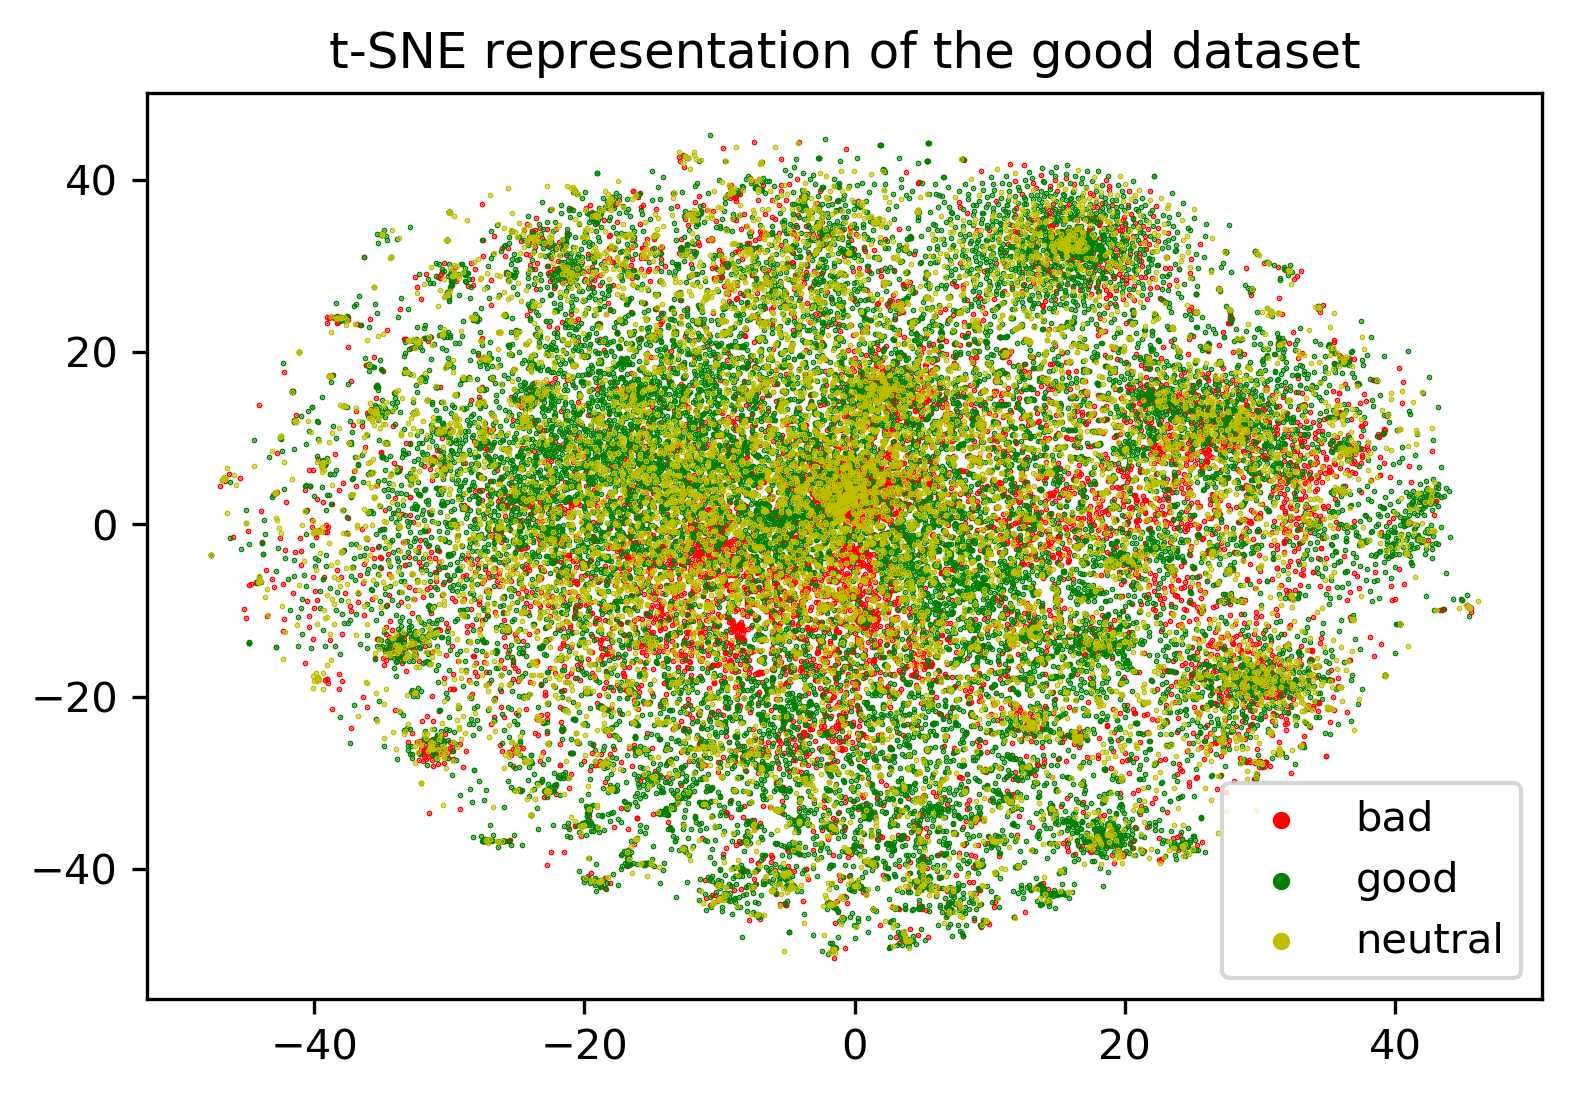
\includegraphics[width=0.5\textwidth]{pics/good.png}
			}%
			\subfigure[bad dataset]{%
				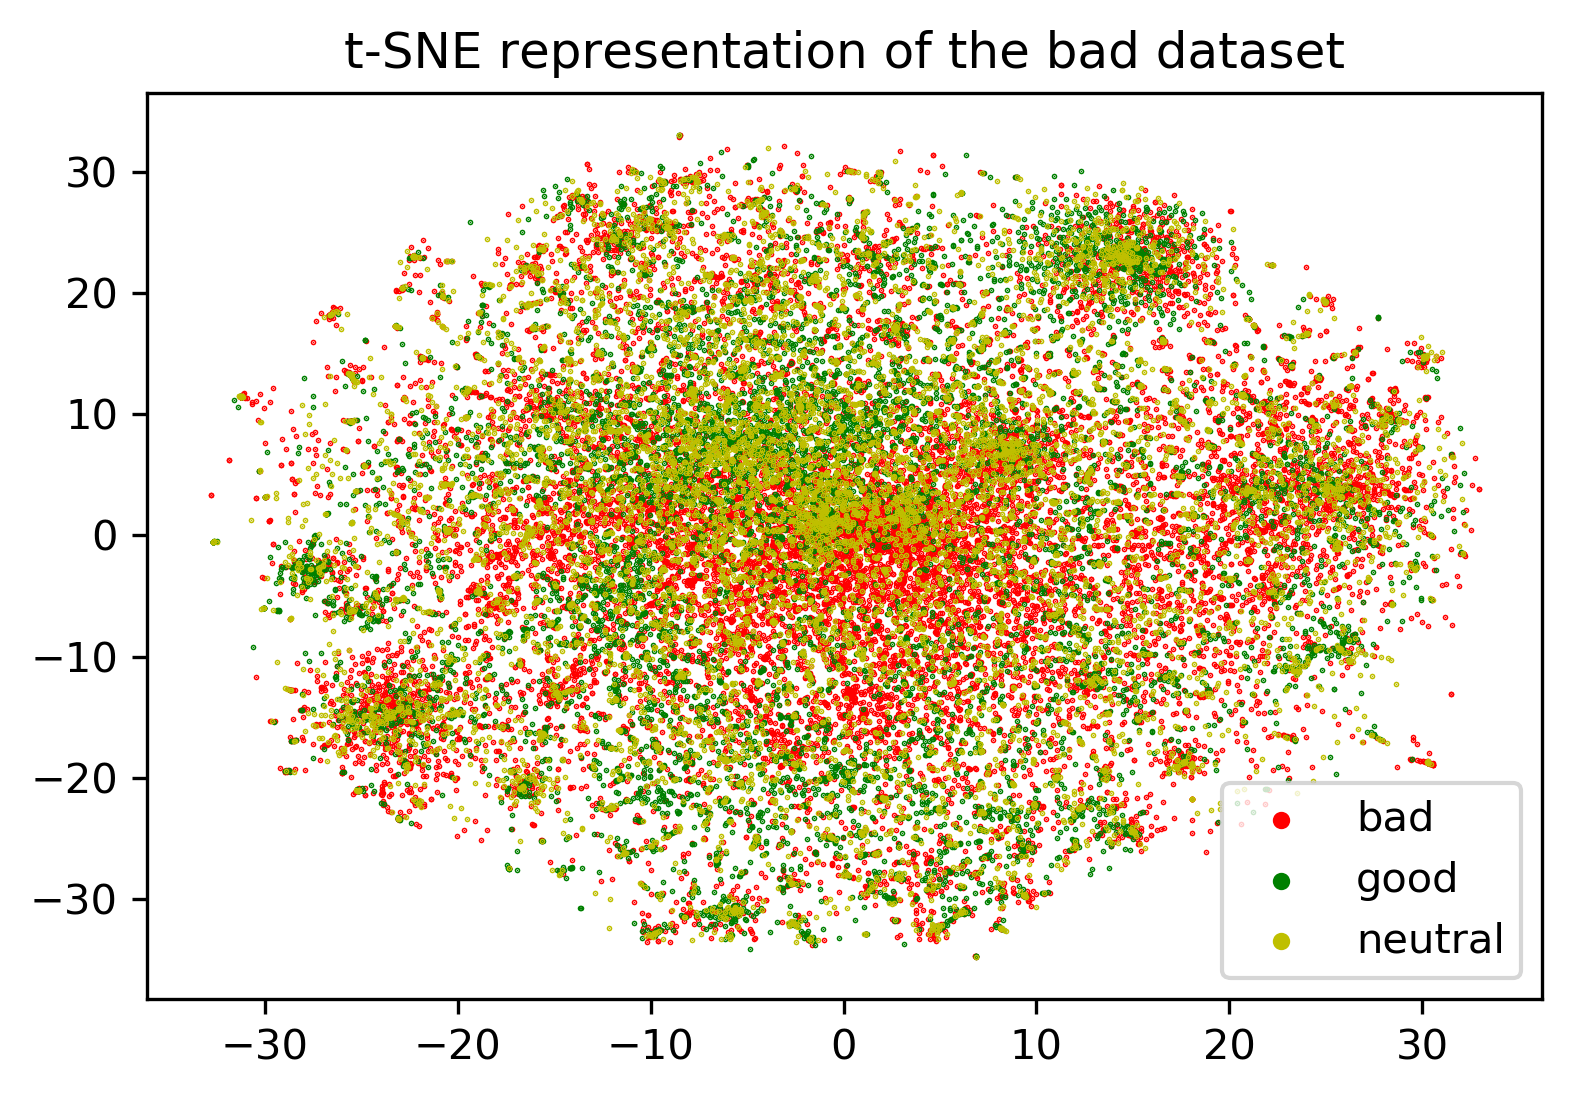
\includegraphics[width=0.5\textwidth]{pics/bad.png}
			}
		\end{center}
\caption{Data visualization after t-SNE with $2$ dimensions}
\label{pic:tsne}
\end{figure}

Figure~\ref{pic:tsne} encourages us to differentiate the analysis and training for \textit{good} and \textit{bad} reviews and hence to design two models who's purpose it is to provide a binary classification if $s_r > 0.80$ -- $r$ is a \textit{good} review -- and a second model that determines if $s_r < 0.20$ -- thus $r$ is a \textit{bad} review. Looking at Figure~\ref{pic:tsne} we can see, that the majority for both \textit{good} and \textit{bad} reviews forms clusters whereas the \textit{neutral} reviews are spread without an underlying structure. Hence deducing decision boundaries for a meaningful separation seems rather difficult. On the other hand we believe that those \textit{neutral} reviews are \textit{neutral} for a reason, the different reader apparently do not agree on if this particular review was helpful after all or not. Also classifying both \textit{good} and \textit{bad} reviews delivers the highest gain of information for Amazon and thus the end customer. 

%\defaulttext{Describe the machine learning problem you have addressed in your mini
%project, your applied method and used data in general terms.}
%%%
%\points{2}

\section{Related work}

There are many proposed solutions for text classification problems. They involve both neural and non-neural techniques. Some of the prior work on Amazon movie reviews has shown that ensemble learning using derived features (like review length, product rating) which performed better in comparison to plain classification methods like SVMs or logistic regression.
Other work used contextual metadata features (like product category, reviewer details) which seemed to work when using non-neural models.

Around 2011, deep networks starting becoming popular after the conception of convolutional neural nets\cite{DBLP:journals/corr/Kim14f} for sentence classification. They started to consistently perform better compared to the conventional classification methods listed above. Gradually when RNNs (recurrent neural nets) came into picture researchers started to take advantage of the architecture. Specifically, the introduction of LSTMs (Long Short-Term Memory Units) started to revolutionize the challenging domains of speech recognition, machine translation and image captioning.

Owing to such growing popularity of LSTMs there were many deep network architectures researched, built and published leveraging multiple-layers of LSTMs for the natural language processing domain. One such notable work is for predicting product review helpfulness using a deep net arch with 2 LSTM layers along with sophisticated NLP features\cite{wei}. 
%%

\section{Method}

Considering the fact that there already are state of the art solutions to this problem of product review helpfulness, that are adopted by the e-commerce world, we approached this problem from an empirical perspective:
\begin{enumerate}
	\item[Step-A:] Choosing an existing model and validating it with updated load of amazon-reviews.
	\item[Step-B:] Replacing modules of the design by using recent ideas in deep learning.
	\item[Step-C:] Analyzing and experimenting by toggling various features.
\end{enumerate}

\underline{\textbf{Step-A}:} As mentioned in previous section, we used Predicting Amazon Product Review Helpfulness \cite{wei}, as our baseline model. This architecture takes advantage of LSTMs which efficiently understand temporal relationships in time sequence data. Specifically, LSTMs serve the purpose of distinguishing word strings in a given product review well.

We started by validating the baseline architecture by using updated amazon product reviews from 24 categories\cite{McATarShiHen15} further described in the Data section. Experimentation process and obtained results are explained in later sections.

\underline{\textbf{Step-B}:} The architecture used is outlined in the Figure below.
\begin{figure}[h!]
	\centering
	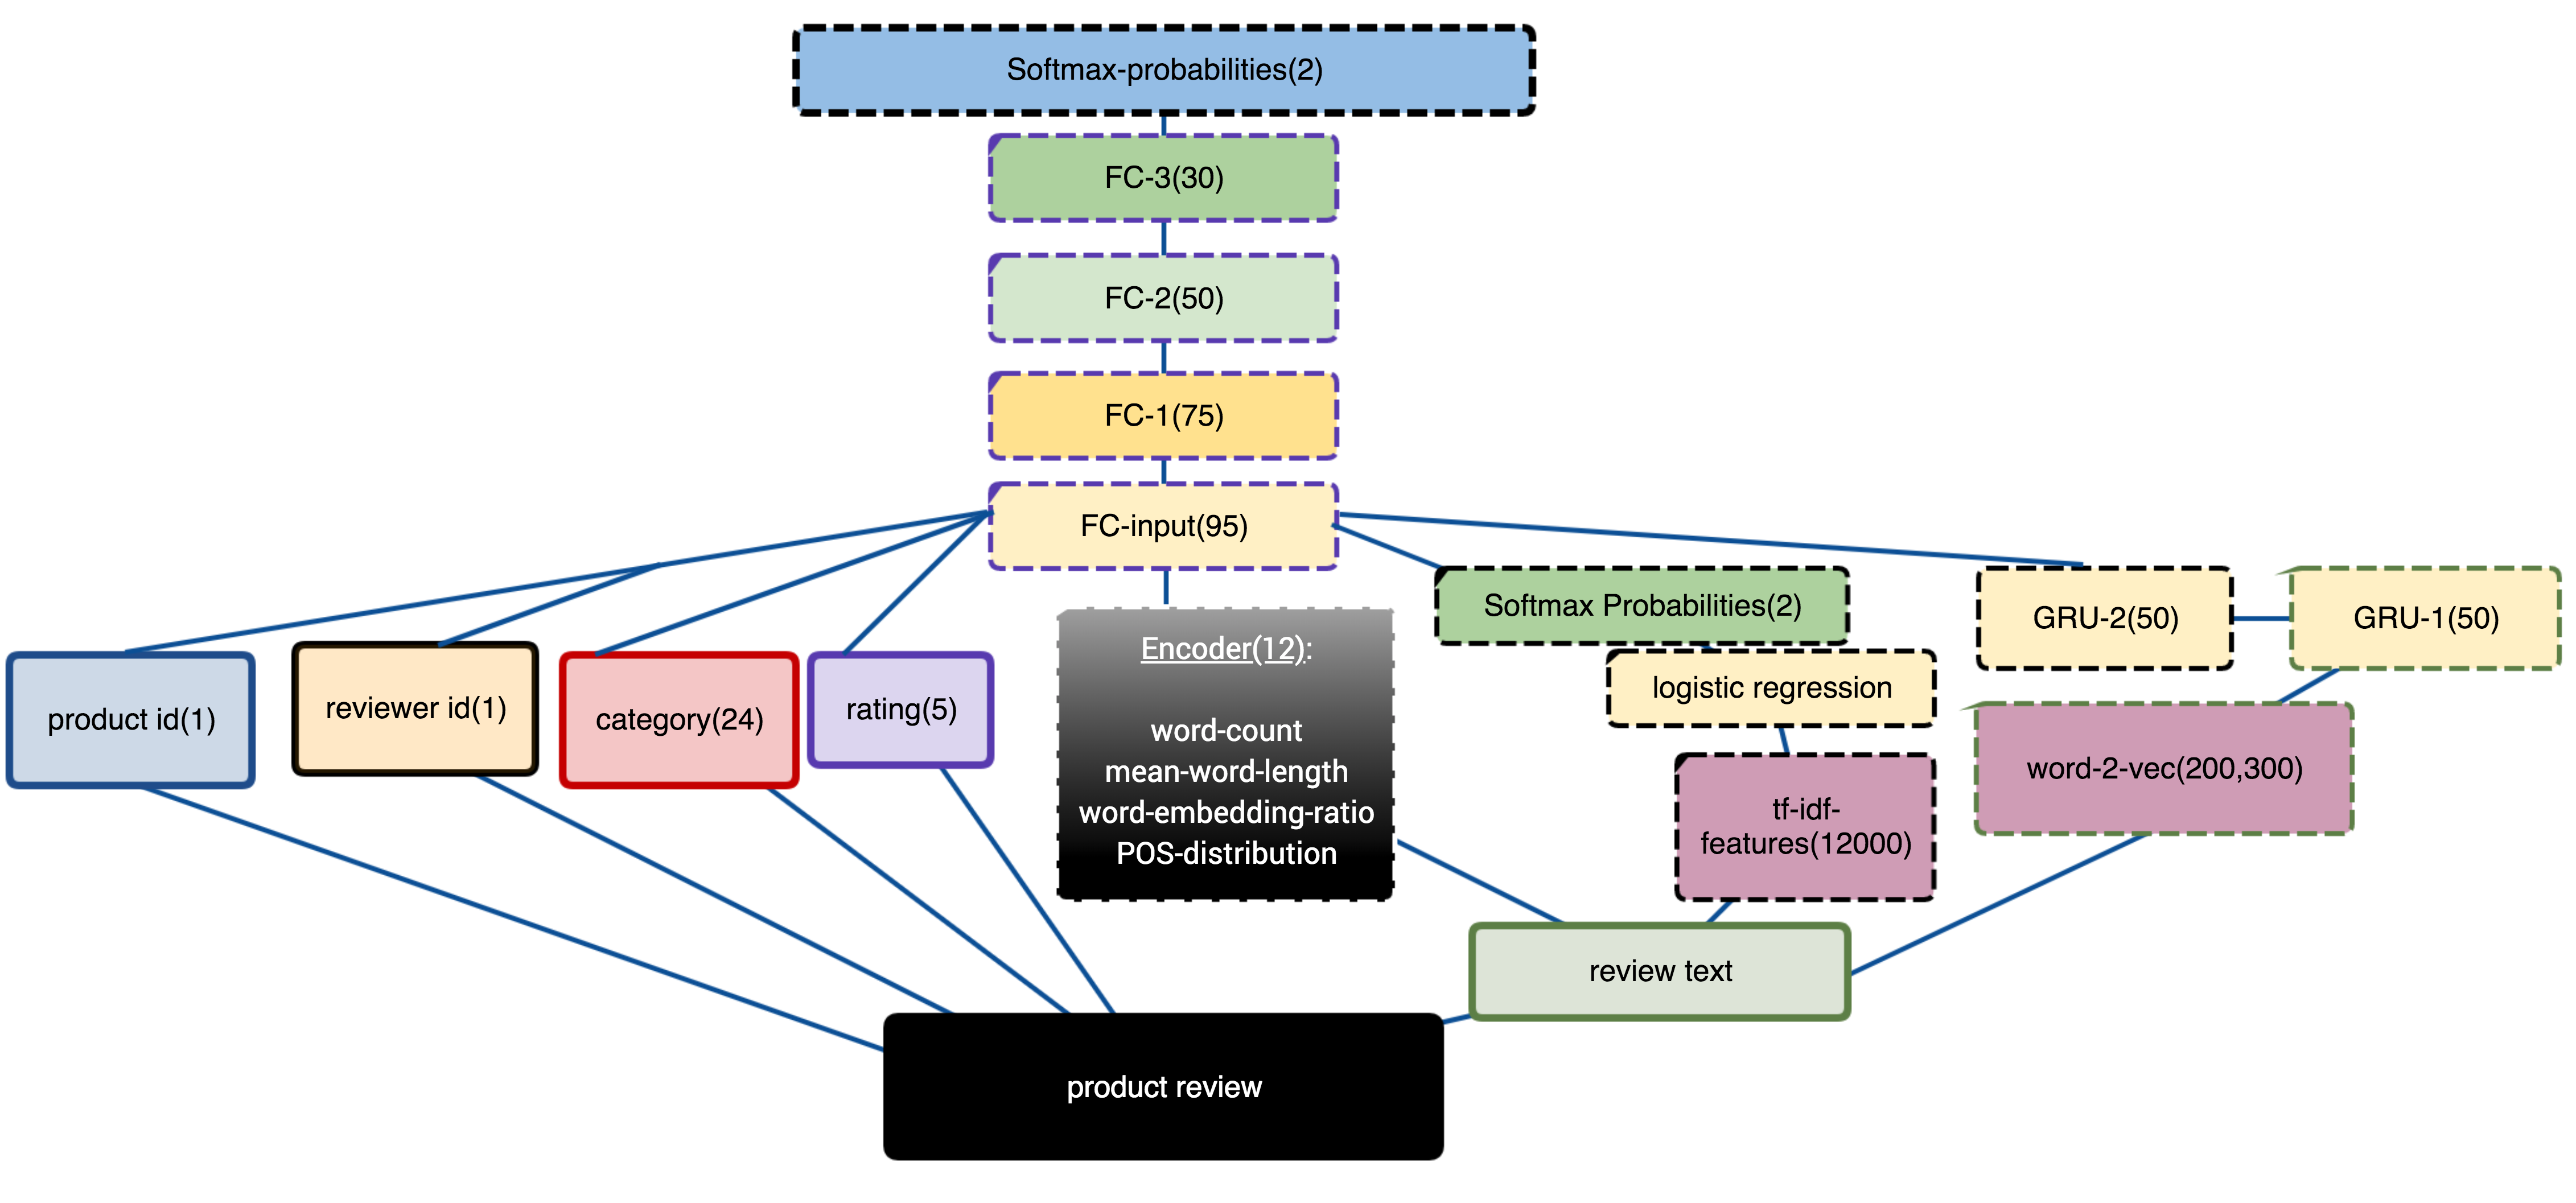
\includegraphics[width=1.05\linewidth]{pics/arch.png}
	\captionsetup{justification=centering,margin=2cm}
	\caption{Modified Network Architecture}
	\label{pic:arch}
\end{figure}

As we know RNNs are designed for handling variable length sequential input by way of shared, recurrent hidden states. They weren't efficient because of the vanishing and exploding gradient issue and the obvious memory constraints until the conception of LSTMs and GRUs (Gated Recurrent Units) at a later point of time. These improved models still solve the same goals of mitigating and tracking long-term dependencies, but more effectively. 

The LSTMs achieve this via the input (regulates how much of the new state to keep), output (regulates amount of the current cell state to be exposed) and forget gates (regulates how much of the existing memory to forget). On the other hand GRUs achieve this by using a reset and update gates. In fact GRUs are basically LSTMs excluding the output gate and thereby the past hidden states are always visible.

\begin{equation}
\boldmath
\begin{cases}
\text{update-gate} = \sigma(\text{review-text-vector} * U^z + s_{t-1}W^z),\\
\text{reset-gate} = \sigma(\text{review-text-vector} * U^r + s_{t-1}W^r)
\end{cases}
\end{equation}

\underline{\textbf{Step-C}:} We start with 95 features before entering the realm of fully connected layers. These are detailed in the \nameref{sec:data} section that follows. We experimented by varying all the hyper-parameters (like the number of GRU cells, number of layers and other regularization attributes of the wrappers extending standard RNNs). The model we used also incorporates some of the methods NLP (natural language processing) toolkit for the purposes of normalizing, standardizing and boosting the training process:
\begin{itemize}
	\item NLTK stop-words removal
	\item Word2Vec embedding
	\item tf-Idf featurization
\end{itemize}

These are explained in the later sections.

%%
%\points{3}

\section{Data}\label{sec:data}
\subsection{Description}

The data used for this mini project is the Amazon product review data by Julian McAuley from UC San Diego \cite{HeM16} \cite{McATarShiHen15}. His data contains Amazon product reviews and metadata, including 142.8 million reviews spanning May 1996 - July 2014.
A product review in the dataset is build up by the following fields: \textit{reviewer ID}, \textit{asin} (product ID), \textit{helpful} (tuple of two integers $f_p$ and $f$), \textit{review Text}, \textit{overall} (rating out of five), \textit{summary} and \textit{category} (like books, electronics or digital music).
An exemplary review is displayed in Table~\ref{tab:JSON}. 

\begin{table}[h!]
\centering
 \begin{tabular}{l |c}
 JSON category & example review value \\ \hline
 reviewer ID & A2B73CL3QSYWLB \\ 
 asin & B000IBUP6A \\ 
 helpful & [3, 6] \\ 
review Text & This film was a minor letdown after reading all the five star reviews ... \\ 
 overall & 4.0 \\ 
 summary & Very Good Crime Film \\ 
 category & Amazon Instant Video
 \end{tabular}
 \captionsetup{justification=centering,margin=2cm}
 \caption{ Exemplary content of a sample review from the Amazon product review dataset}
 \label{tab:JSON}
\end{table}

A reduced 5-core version of the dataset can be downloaded from the \href{http://jmcauley.ucsd.edu/data/amazon/links.html}{website of Julian McAuley}. In the 5-core dataset each product review and user has at least five entries, which contains in total 18.2 million reviews. Additionally we filtered our reviews which had less than five helpfulness feedback votes, which reduces the remaining dataset to 3.0 million reviews.

\begin{figure}[h!]
\centering
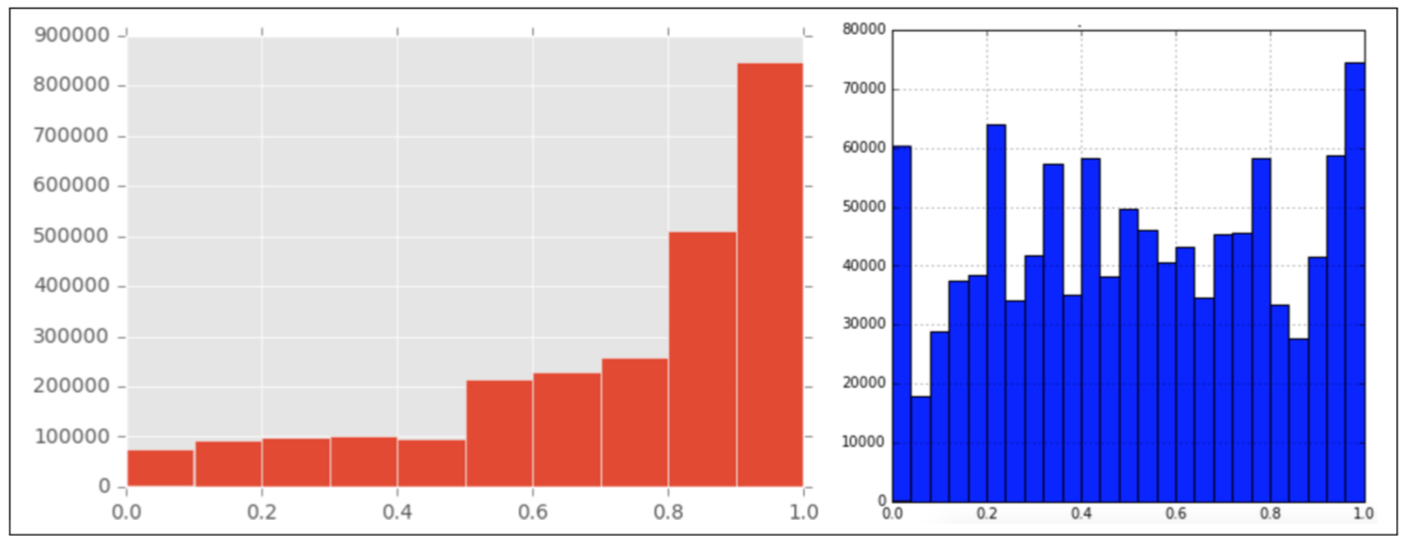
\includegraphics[width=0.7\linewidth]{pics/data_distribution.png}
\captionsetup{justification=centering,margin=2cm}
\caption{Distribution of helpfulness scores: \\ (left) for the filtered 5-core dataset, (right) after unskewing}
\label{pic:distri}
\end{figure}

After leaving out reviews with less than five helpfulness feedback votes we saw, that the distribution of helpfulness scores is not equally distributed but rather skewed, as nearly half of the 3.0 million reviews have a helpfulness score of greater than 0.8. This is displayed in Figure~\ref{pic:distri}. 

In order to evenly distribute the dataset the entire range of the helpfulness score, we unskewed the data by randomly selecting the same number of reviews within a 0.2 helpfulness-score-bucket. The process of unskewing left 1.1 million reviews roughly uniformly distributed in the final dataset.

After we tried to further analyze the full dataset we ran into memory issues as both machines in \textit{Paniikki} as well as servers such as \textit{force} couldn't cope with the vast number of reviews, which is why we decided to reduce the data by randomly sampling a subset of 50,000. 80\% of this dataset are used for both training and validation and the remaining 20\% are used for the final test.

\subsection{Preprocessing}

In order to standardize the raw text of all reviews we transformed the raw text into normalized 1-grams. The raw text is the concatenation of the \textit{summary} field and the \textit{reviewText} field. 
Additionally we preprocessed the data with the following operations:

\begin{enumerate}[(i)]
\item remove all capitalization
\item tokenize the text and remove whitespace, symbols, punctuation, numerals
\item for all tokens, we filtered out:
\begin{itemize}
\item English stopwords (according to the NLTK stopwords corpus)
\item tokens with less than three characters
\end{itemize}
\end{enumerate}

%\defaulttext{Tell where the data is from, what it contains, the number of samples
%in training, validation and test sets, the dimensional, etc.  Also
%describe the preprocessing stages applied by the providers of the data
%or by you yourselves.}
%%
%\points{3}

\section{Experiments}

%\defaulttext{Explain the goal and implementation of your experiments.  Tell what
%hyperparameters values you experimented with and what other
%variations in the method you tested.}
%%%
%\points{5}

As stated in our methodology, we started evaluating baseline models to prove their assertions true. We found a convincing architecture which performed well on the test set, so we proceeded to implement in \textit{TensorFlow}. This library has the advantage, that many modules are already implemented. We also used \textit{nltk} for word stemming, \textit{gensim} for word embedding, \textit{pandas} to handle the datasets, \textit{sk-learn} for t-SNE computation and \textit{matplotlib} for visualizations.

The schema implemented is explained next. The design variations are discussed following to it.

\subsection{Main model framework}\label{sec:main_model_framework}
The approach, is displayed in Figure \ref{pic:arch}. At the end we have one set of fully-connected layers with a softmax function. They are configured with length $75, 50$ and $30$, leakyRELU ($max(0.01x, x)$) as the activation function and dropout \cite{dropout:JMLR:v15:srivastava14a} as regularization. This network is fed with a number of high-level input features. Namely:
\begin{description}
	\item[Product id, reviewer id, category, rating] We wanted to take into account the crucial relations of the product reviews with their source; the reviewer themself. I.e. If a reviewer explains their thoughts more concisely than others. For that purpose we feed the network with those labels, taken directly from the dataset.
	
	The category also makes sense to appear, as some reviewers have more expertise than others on certain areas, which allows them to produce higher-quality reviews.
	
	The rating is also evident, as it's the numerical opinion of the product by the reviewer.
	
	\item[Anatomical encoder] We used an encoder to extract common Natural Language Processing features we found valuable in the baseline model, like the number of tokens, the length of those, the number of characters in the token, etc. Which are produced by using techniques like:
	\begin{itemize}
		\item \textbf{Tf-idf featurization} \cite{tfidf:Ramos2003UsingTT} a statistic to measure how important a word is regarding the whole document. Which internally uses \textit{uni-gram normalization}.
		\item \textbf{Stemming} to reduce words to they root form, and use them as tokens.
		\item \textbf{Word2vec} \cite{word2vec:DBLP:journals/corr/abs-1301-3781} Word embeddings that produce a vector space, with each word corresponding to a vector in that space. Words that are related on a context are positioned close to each other. This help us creating a useful representation of the words.
	\end{itemize}
	
	\item[Logistic regression] We applied logistic regression with $l_2$ regularization to the td-idf features of the top 12.000 text reviews words, stemmed to reduce the set of $n$-grams to consider. We have two regression models to classify good and bad reviews respectively. There is only one hyper-parameter, a regularization variable to avoid overfitting. With simple binary search we could find the optimal value at $1$ for the good reviews dataset and $0.23$ for the bad reviews one.
	
	\item[Recurrent networks] A well known recurrent neural network was used for modelling the temporal data, \textit{Long Short-Term Memory} nets \cite{Hochreiter:1997:LSM:1246443.1246450}. It was fed with a pre-trained \textit{word2vec} model of the reviews. We used 50 units for the configuration, the regularization method was \textit{dropout} and we applied \textit{Adam} \cite{adam:DBLP:journals/corr/KingmaB14} parameter optimizer.
\end{description}

After understanding, implementing and engineering the model training to use \textit{Paniikki} machines, we started with our own variations to try to improve the baseline performance or accuracy. The most important ones are mentioned in the following subsections.

\subsection{GRUs}
LSTMs are just one type of recurrent cell. There are a wide range of different ones, with their own pros and cons. As explained in the methods section, we took into consideration Gated Recurrent Units \cite{gru:DBLP:journals/corr/ChungGCB14} (GRUs) because it seemed most appropriate.

We used the same configuration as for the LSTM units, with the same optimizer (Adam).

\subsection{Parameter variations}
We varied the following parameters and hyper-parameters of the neural network:
\begin{itemize}
	\item The number of units in each GRU cell. Ranging from 25 to 95 units with a step interval of 10, before concluding for 50.
	\item The number of GRU layers. The base paper empirically proved that 2 layered LSTM performed well in comparison to a single one. We started with the same premise and validated the same. We also noticed that increasing the number of layers further did not have any impact on the results, but increased the time required for training drastically. A reason we inferred for this is relies on the constraints of the number of features.
\end{itemize}

\subsection{Features relevance}
During the implementation, we questioned the utility of \textit{product id} and \textit{reviewer id} context features. We thought that feed some identifiers to the network don't make any sense. We tried to train the model without those features, which resulted into worse accuracy.

\section{Results}

\defaulttext{Give the results of your experiments in a table and explain them in
	the text.  Some figures would be good here for illustration.  Refer to
	the table(s) and image(s) in the text and describe them.}
%%
\points{5}

table: time  performance
lstms
grus
nlp features

\subsection{LSTM vs GRU}

\section{Discussion}

\defaulttext{Discuss your results in comparison with comparable results your have
found in the literature and web.  Explain any other findings you made
while running the experiments.}
%%
\points{4}

\section{Conclusions}

This mini project consists in the comparison and improvement of the existing LSTM model \cite{wei} and shows, that using GRU instead of LSTM by itself is reflecting in improved results. 
 
Firstly we had to take care of the heavily skewed dataset towards good reviews, which we did by unskewing the data. This steps enables every deep learning model applied to this dataset to correctly learn the underlying importance of features rather than just reflecting the dominating presence of good reviews.

Overall the results show, that a binary classification for good reviews is more accurate than the classification for bad reviews. This is not that surprising after all, as helpful reviews tend to be both well structured and well written in terms of vocabulary. Bad reviews on the other hand are generally shorter and written in a less extensive way. Thus the model for the good reviews has more characteristics it can learn from. This point is also backed up by the t-SNE representation of the data displayed in Figure~\ref{pic:tsne}. The cluster representation of the good reviews is slightly sharper defined than the one representing bad reviews.

%\defaulttext{Give your final conclusions from the whole mini project and its results.}
%%
%\points{3}

\section{References}
\bibliography{bibliography}{}
\bibliographystyle{acm}
%%
%\points{2}

\section{Roles of the authors}

This mini project was designed to \textit{allow the students to use the theoretical knowledge gained during the course in real life practical machine learning challenges}. In order to fully accomplish this main goal we tried to always work as a team and participate in all tasks equally.

Regardless of this overall working principle we summarize the main tasks each member was involved in in Table~\ref{tab:roles}. This list contains only the most important responsibilities and must not be mistaken with an overarching list of tasks and responsibilities.

\begin{table}[bh!]
\centering
 \begin{tabular}{l |l}
 member 		& task \\ \hline
 Aditya		&  dataset analysis, architecture of DL model, data gathering, visualization, \\ 
 			& word embedding , measure accuracy, anatomical feature, reporting,  \\
			& scheduling tasks, debugging, remote server access\\ \hline
 H�ctor 		&  remote server access, data gathering, measure accuracy, dataset analysis,\\
 			& anatomical feature, reporting, word embedding, scheduling tasks, debugging, \\
			& architecture of DL model, visualization\\ \hline
 Maximilian 	& word embedding ,reporting, anatomical feature, remote server access,\\
 			& measure accuracy, data gathering, dataset analysis, visualization, \\
			& architecture of DL model, scheduling tasks, debugging
 \end{tabular}
 \captionsetup{justification=centering,margin=2cm}
 \caption{Involvement of main tasks and responsibilities broken down to the team members}
 \label{tab:roles}
\end{table}

%\defaulttext{If you have more than one member in your mini project group, you need
%to explain in this section how the labor was divided between you and
%what were each one's roles in the project and its reporting.}

\end{document}